%\section{Introduction}
%\label{sec:intro}

Modelling is fundamental to the success of technological innovations for artificial intelligence. A powerful model learns a useful representation of the observations for a specified prediction task, and generalises to unknown instances that follow similar generative mechanics. 
%
A well established area of machine learning research focuses on developing \emph{prescribed probabilistic models} \citep{diggle:prescribe_implicit1984}, where learning is based on evaluating the probability of observations under the model. \emph{Implicit probabilistic models}, on the other hand, are defined by a stochastic procedure that allows for direct generation of samples, but not for the evaluation of model probabilities. These are omnipresent in scientific and engineering research involving data analysis, for instance ecology, climate science and geography, where simulators are used to fit real-world observations to produce forecasting results. 

Within the machine learning community, there is a recent interest in a specific type of implicit models, generative adversarial networks (GANs) \citep{goodfellow:gan2014}, which has been shown to be one of the most successful approaches to image generation \citep{radford:dcgan2016, arjovsky:wgan2017, berthelot:began2017}. Very recently, implicit distributions have also been considered as approximate posterior distributions for Bayesian inference, e.g.~see discussions in the last chapter and recent papers including \citet{liu:two_wild2016, wang:amortisedsvgd2016, karaletsos:adversarial_mp2016, mescheder:avb2017, huszar:implicit2017, li:amcmc2017, tran:implicit2017, shi:kivi2018}. These examples demonstrate the superior flexibility of implicit models, which provide highly expressive means of modelling complex data structures.


%Many machine learning papers mainly focus on developing \emph{prescribed probabilistic models} \citep{diggle:prescribe_implicit1984} for their tasks, where learning is usually done by evaluating the probability of observations under the model. However, \emph{implicit probabilistic models}, which are defined by a stochastic procedure that directly generates samples, have also attracted major attention. In many scientific fields that involve data analysis, for instance ecology, climate science and geography, simulators are commonly used to fit the real-world data and produce forecasting results. Another example of such implicit models are generative adversarial networks (GAN) \citep{goodfellow:gan2014} which have been shown to be one of the most successful approaches to image and text generation \citep{radford:dcgan2016, yu:seqgan2017, arjovsky:wgan2017, berthelot:began2017}. Very recently, implicit distributions have also been considered as approximate posterior distributions for Bayesian inference, e.g.~see \citep{liu:two_wild2016, wang:amortise_svgd2016, li:wild2016, karaletsos:adversarial_mp2016, mescheder:avb2017, huszar:implicit2017, li:amcmc2017, tran:implicit2017}. These examples demonstrate the superior flexibility of implicit models, which are highly expressive in modelling many data structures.

Whilst prescribed probabilistic models can be learned by standard (approximate) maximum likelihood or Bayesian inference, implicit probabilistic models require substantially more severe approximations due to the intractability of the model distribution. Many existing approaches first approximate the model distribution or optimisation objective function and then use those approximations to learn the associated parameters. However, such approximation can lead to unstable training and poor results, where a prevalent example is the original GAN framework \citep{goodfellow:gan2014} that has been briefly sketched in Section \ref{sec:chap5_grad_approx}.
%
Recent ideas to address this issue for GANs suggest that restricting the representational power of the discriminator is effective in stabilising training \citep[e.g. see][]{arjovsky:wgan2017, kodali:dragan2017}. However, such restrictions, if not carefully crafted, often introduce undesirable biases, responsible for problems such as mode collapse in the context of GANs, and uncertainty underestimation in variational inference methods \citep{turner:two_problems2011}.

\begin{figure}
\subfigure[approximate loss function \label{fig:approx_loss}]{
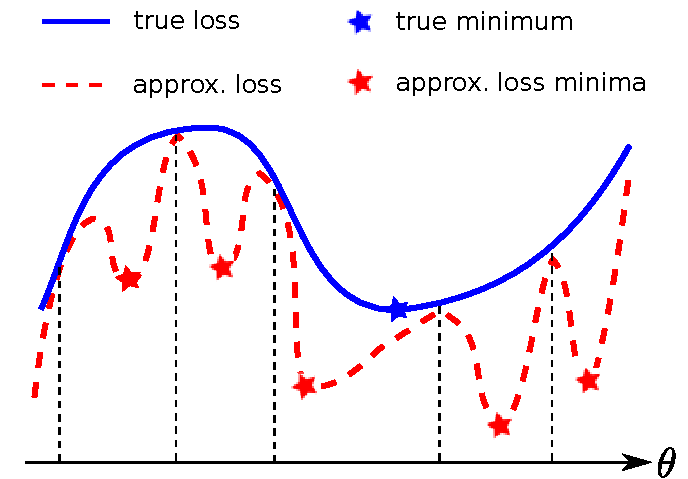
\includegraphics[width=0.45\linewidth]{figs/approx_loss.pdf}}
\hfill
\subfigure[approximate gradients \label{fig:approx_gradient}]{
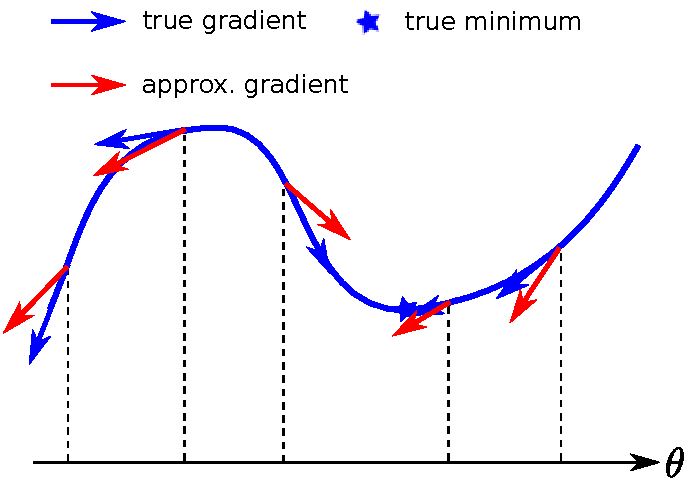
\includegraphics[width=0.45\linewidth]{figs/approx_gradient.pdf}}
\caption{A comparison between the two approximation schemes. Since in practice the optimiser only visits finite number of locations in the parameter space, it can lead to over-fitting if the neural network based functional approximator is not carefully regularised, and therefore the curvature information of the approximated loss can be very different from that of the original loss (shown in (a)). On the other hand, the gradient approximation scheme (b) can be more accurate since it only involves estimating the sensitivity of the loss function to the parameters in a local region.}
\label{fig:loss_grad_approx_compare}
\end{figure}

%Whilst prescribed probabilistic models can be learned by standard approximate maximum likelihood or Bayesian inference, implicit probabilistic models require more severe approximations due to the intractability of the model distribution. Many existing approaches first approximate the model distribution and/or optimisation objective functions, then learn the associated parameters using the defined approximations. For example, GANs use a discriminator which serves as a critic of the generative model, and let both networks play a minimax game until convergence. However, for finite number of data-points, there are infinite number of functions that could perfectly approximate the exact objective function evaluated at those observations, and for some of these approximating functions the gradient directions can be arbitrary far away from the exact ones. This is especially true when the approximated objective function is represented by neural network critics, where recent advances for stabilising GANs suggest restricting the representation power of the discriminator (e.g. see \citep{arjovsky:wgan2017}). There exist similar issues for variational methods as well, i.e.~proposing a lower-bound/upper-bound to the exact loss function. Similar to the variational lower-bound, these bounds are unlikely to be equally tight everywhere \citep{turner:two_problems2011}. It often biases the approximate posterior towards under-estimating uncertainty, and similarly for GANs the same problem exists as mode collapsing.

In the previous chapter a number of proposals for wild approximate inference are presented. Critically, we believe these techniques are extendable to learning implicit models, and in this chapter we explore the \emph{direct gradient approximation} idea as an alternative. A visualisation of the two approximation schemes is provided in Figure \ref{fig:loss_grad_approx_compare}. More specifically we focus on approximating the score function, in which an accurate approximation of it then allows the application of many well-studied algorithms, such as maximum likelihood, maximum entropy estimation, variational inference and gradient-based MCMC, to implicit models. Concretely, our contributions include:  
\begin{itemize}
\item the \emph{Stein gradient estimator}, a novel generalisation of the score matching estimator \citep{hyvarinen:score2005}, with both parametric and non-parametric versions;
\item a comparison of the proposed estimator with the score matching and the KDE plug-in estimators on performing gradient-free MCMC, meta-learning of approximate posterior samplers for Bayesian neural networks, and entropy based regularisation of GANs.
\end{itemize}

%In this paper we explore an alternative idea of training implicit models, which directly approximates the gradient of the implicit model distribution. More precisely we focus on approximating the score function $\nabla_{\x} \log q(\x)$ for some distribution $q$ to be learned. The score function is widely used in machine learning algorithms, e.g.~maximum likelihood, variational inference and gradient-based MCMC. Hence an accurate approximation to the score function would enable the application of these well-studied algorithms to implicit models. After reviewing recent advances in implicit models and gradient approximation techniques, we make the following contributions:  
%\begin{itemize}
%\item We propose the \emph{Stein gradient estimator} as a novel generalisation of the score matching estimator \citep{hyvarinen:score2005}, with both parametric and non-parametric versions presented;
%\item We compare the Stein estimator with the score matching estimator and the KDE plug-in estimator on three different tasks: gradient-free MCMC, entropy regularised GANs, and meta-learning of approximate posterior samplers for Bayesian neural networks.
%\end{itemize}